\documentclass[11pt,a4paper]{article}
\usepackage[margin=2.6cm]{geometry}
\usepackage{amsmath,amssymb}
\usepackage{booktabs}
\usepackage{array}
\usepackage{enumitem}
\usepackage{xcolor}
\usepackage{tikz}
\usepackage{pgfplots}
\pgfplotsset{compat=1.17}
\usepackage[colorlinks=true,linkcolor=teal!70!black,citecolor=teal!70!black,urlcolor=teal!70!black]{hyperref}

\definecolor{bandA}{HTML}{008A7C}
\definecolor{bandB}{HTML}{C2610C}
\newcommand{\tagbox}[2]{\textsf{\scriptsize\colorbox{#1!12}{\textcolor{#1!70!black}{#2}}}}
\newcommand{\est}{\tagbox{gray}{established}}
\newcommand{\lit}{\tagbox{blue}{literature}}
\newcommand{\ours}{\tagbox{orange}{ours}}
\newcommand{\lP}{\ell_{\mathrm P}}

\title{Counting Neighbours in a Discrete Spacetime\\[4pt]
\large Lorentz invariance, quantum blur, finite universes and the creation of points}
\author{Draft --- internal notebook checkpoint}
\date{24 October 2026 \\[2pt] \small Not for circulation. Every claim is tagged \est, \lit{} or \ours.}

\begin{document}
\maketitle

\begin{abstract}
We explore, at an elementary level, the hypothesis that spacetime is a discrete set of points that only looks like a smooth Lorentzian manifold when viewed from far away. Defining two points as \emph{neighbours} when information can pass between them in one ``tick'' of proper time, we show by direct counting that any discrete structure with boost symmetry---random or crystalline---gives every point infinitely many neighbours, while any structure with finitely many neighbours singles out a preferred frame. This reproduces, by sophomore-level means, a known result of causal set theory. We then examine three ways of softening the dilemma: (i) ``quantum blurring'' of the points, which we show cures the zero-measure problem but not the divergence, and which runs into a recurring obstruction we summarise as \emph{normalisable states cannot be boost-invariant}; (ii) a finite universe, which cuts the divergence off at a rapidity $\eta_{\max}\approx\ln(2L/\lP)\approx 142$, far above the largest rapidity ever observed ($\approx 27$); and (iii) a ``point budget'' in which cosmic expansion creates points and gravitating matter destroys them. A toy quantum chain shows that zero-point motion gives each point a collective positional blur that grows as $\ln N$ in one dimension and saturates in three. We are explicit about what is known, what may be new, and what is likely wrong.
\end{abstract}

\section{Motivation}
In 1900 Planck assumed, as ``an act of desperation'', that energy is exchanged in discrete quanta. The analogous move for spacetime is to assume it is a discrete set of points and to recover the smooth manifold of general relativity (GR) as a large-scale limit, \emph{before} attempting quantisation. This ``discrete first'' ordering is the founding philosophy of causal set theory~\cite{BLMS87}; discreteness also appears as a derived result in loop quantum gravity and as a regulator in causal dynamical triangulations~\cite{AJL05}.

Our aim here is not a new theory. It is to work through the idea with elementary tools, see which walls appear, and record which small observations might be our own. Throughout, claims are tagged \est{} (tested mainstream physics), \lit{} (published, not necessarily accepted) or \ours{} (our speculation or construction).

\section{Discrete things that look continuous}
\paragraph{The atomic chain.} \est{} Masses $m$ joined by springs $\kappa$ at spacing $a$ obey $m\ddot u_n=\kappa(u_{n+1}-2u_n+u_{n-1})$. Taylor-expanding $u_{n\pm1}=u(x\pm a)$,
\begin{equation}
\ddot u=c^2u''+\frac{c^2a^2}{12}u''''+\dots,\qquad c^2=\frac{\kappa a^2}{m},
\end{equation}
so in the limit $a\to0$ at fixed $c$ we recover the wave equation with a finite signal speed. The exact dispersion relation $\omega=(2c/a)|\sin(qa/2)|$ gives a group velocity $c\cos(qa/2)<c$: short waves are slower, the classic signature of discreteness.

\paragraph{Regular lattices give polygons, not circles.} \lit{} If ``neighbour'' means ``reachable in one hop per tick'', the set reached after $N$ ticks is the light cone. On a square lattice it is the diamond $|x|+|y|\le N$; on a hexagonal lattice, a hexagon. Burago's theorem states that any periodic metric rescales to a \emph{norm}, and for lattices with step-counting the unit ball is a polygon~\cite{Burago}. This is the rigorous form of Weyl's tile argument~\cite{Weyl}: a crystal predicts a direction-dependent speed of light at all scales. Random graphs escape: first-passage distances on Poisson--Voronoi tessellations converge to an exact Euclidean ball~\cite{VahidiAslWierman}. \emph{Randomness buys isotropy.}

\section{The neighbour problem}
Work in $1+1$ dimensions with $c=1$. Call $x$ a one-tick neighbour of the origin if it lies in the future with proper time $0<\tau<\varepsilon$.

\subsection{The sliver}
The neighbour region is the sliver $0<t^2-x^2<\varepsilon^2$, $t>0$, between the light cone and the hyperbola (Fig.~\ref{fig:sliver}). With light-cone coordinates $u=t-x$, $v=t+x$ one has $t^2-x^2=uv$ and $dt\,dx=\tfrac12du\,dv$, so
\begin{equation}
A=\frac12\int_0^\infty du\int_0^{\varepsilon^2/u}dv=\frac{\varepsilon^2}{2}\int_0^\infty\frac{du}{u}=\infty .
\end{equation}
Restricted to $|x|\le X$ the area is $X\sqrt{X^2+\varepsilon^2}-X^2+\varepsilon^2\ln\frac{X+\sqrt{X^2+\varepsilon^2}}{\varepsilon}\approx \tfrac{\varepsilon^2}{2}+\varepsilon^2\ln\frac{2X}{\varepsilon}$: the sliver thins like $\varepsilon^2/2x$, and its area grows like the harmonic series.

\subsection{Rapidity bands: the conveyor belt}
\ours{} (pedagogical form of a known fact). Write $u=\tau e^{-\eta}$, $v=\tau e^{\eta}$, so that $x=\tau\sinh\eta$, $t=\tau\cosh\eta$ and $dt\,dx=\tau\,d\tau\,d\eta$. A band of unit rapidity width has area $\int_0^\varepsilon\tau\,d\tau=\varepsilon^2/2$. A boost shifts $\eta$ and maps each band exactly onto the next. The sliver is therefore infinitely many boost-copies of one finite piece. In Euclidean space, rotations act on the annulus with \emph{finitely} many copies because the angle stops at $2\pi$; rapidity never stops.

\begin{figure}[t]
\centering
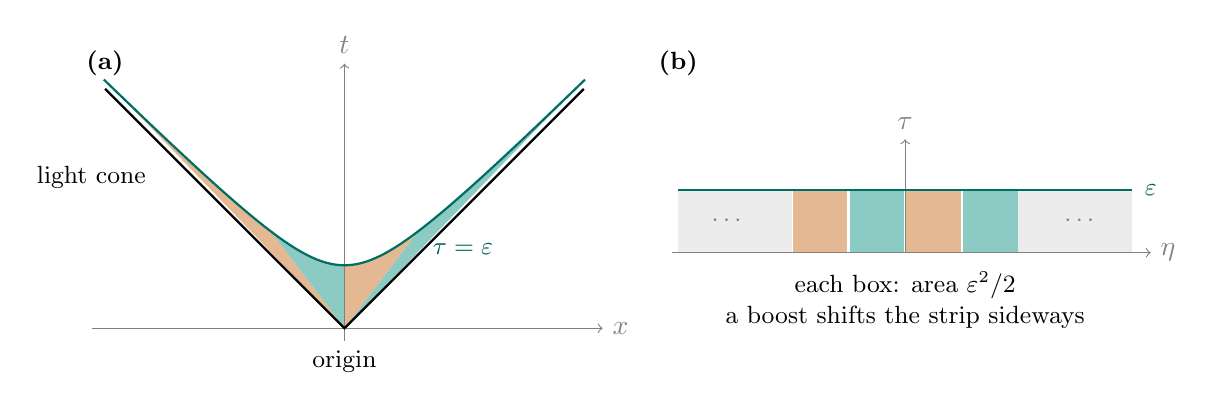
\begin{tikzpicture}[scale=0.8]
  % (a) spacetime picture
  \begin{scope}
  \foreach \a/\b/\c in {-2/-1/bandB, -1/0/bandA, 0/1/bandB, 1/2/bandA}{
    \fill[\c!45] (0,0) -- plot[domain=\a:\b,samples=40,variable=\e] ({sinh(\e)},{cosh(\e)}) -- cycle;
  }
  \draw[->,gray] (-4,0) -- (4.1,0) node[right] {$x$};
  \draw[->,gray] (0,-0.2) -- (0,4.2) node[above] {$t$};
  \draw[thick] (-3.8,3.8) -- (0,0) -- (3.8,3.8);
  \draw[thick,bandA!80!black] plot[domain=-2.05:2.05,samples=80,variable=\e] ({sinh(\e)},{cosh(\e)});
  \node[font=\small,anchor=east] at (-3.0,2.4) {light cone};
  \node[font=\small,bandA!70!black,anchor=west] at (1.25,1.25) {$\tau=\varepsilon$};
  \node[font=\small,anchor=north] at (0,-0.2) {origin};
  \node[font=\small\bfseries] at (-3.8,4.2) {(a)};
  \end{scope}
  % (b) the same region in (eta, tau) coordinates
  \begin{scope}[xshift=8.9cm,yshift=1.2cm]
  \foreach \a/\c in {-2/bandB,-1/bandA,0/bandB,1/bandA}{
    \fill[\c!45] (\a*0.9,0) rectangle ({(\a+1)*0.9},1);
    \draw[white,thick] (\a*0.9,0) -- (\a*0.9,1);
  }
  \fill[gray!15] (-3.6,0) rectangle (-1.8,1);
  \fill[gray!15] (1.8,0) rectangle (3.6,1);
  \node[gray,font=\small] at (-2.8,0.5) {$\cdots$};
  \node[gray,font=\small] at (2.8,0.5) {$\cdots$};
  \draw[->,gray] (-3.7,0) -- (3.9,0) node[right] {$\eta$};
  \draw[->,gray] (0,0) -- (0,1.8) node[above] {$\tau$};
  \draw[thick,bandA!80!black] (-3.6,1) -- (3.6,1);
  \node[font=\small,anchor=west,bandA!70!black] at (3.65,1) {$\varepsilon$};
  \node[font=\small,align=center] at (0,-0.75) {each box: area $\varepsilon^2/2$\\a boost shifts the strip sideways};
  \node[font=\small\bfseries] at (-3.6,3.0) {(b)};
  \end{scope}
\end{tikzpicture}
\caption{(a) Neighbours of the origin lie in the sliver between the light cone and the hyperbola $\tau=\varepsilon$. Each coloured piece spans one unit of rapidity; far from the origin the pieces become too thin to see, but they never end. (b) The same sliver in coordinates $(\eta,\tau)$: an infinite strip of identical boxes, each of area $\varepsilon^2/2$ (since $dt\,dx=\tau\,d\tau\,d\eta$). A boost slides the strip sideways like a conveyor belt. (Interactive version in the notebook.)}
\label{fig:sliver}
\end{figure}

\subsection{``Exactly one tick''}
A natural objection is that discrete time should mean neighbours at \emph{exactly} one tick. The conclusion survives every reading.
\begin{enumerate}[leftmargin=*]
\item \lit{} \emph{Random points.} A curve has zero area, so exact equality gives no neighbours. The natural discrete notion is a causal-set \emph{link}: no other point lies causally between the two. The causal interval of a point at proper time $\tau$ has area $\tau^2/2$, so for a Poisson density $\rho$, $P(\text{link})=e^{-\rho\tau^2/2}$ and
\begin{equation}
\langle N_{\rm links}\rangle=\int d\eta\int_0^\infty\rho\,\tau\,e^{-\rho\tau^2/2}d\tau=\int d\eta\cdot 1=\infty .
\end{equation}
Exactly one expected link per unit rapidity, with no arbitrary $\varepsilon$. Infinite valency is standard in causal set theory~\cite{Surya19,Sorkin11}.
\item \est{} \emph{Square lattice.} $t^2-x^2=k$ means $(t-x)(t+x)=k$, which has finitely many integer solutions. For $k=1$ only $(1,0)$ qualifies. Finite valency, and no boost symmetry at all.
\item \lit/\ours{} \emph{Lattice with discrete boosts} (Schild~\cite{Schild48}). In $2+1$ dimensions with metric $\mathrm{diag}(1,-1,-1)$, the integer matrix
$\Lambda=\left(\begin{smallmatrix}3&2&2\\2&1&2\\2&2&1\end{smallmatrix}\right)$ preserves $t^2-x^2-y^2$ and is a boost with $\cosh\eta=3$. The orbit $(1,0,0)\to(3,2,2)\to(17,12,12)\to\cdots$ gives infinitely many points at exactly one tick.
\end{enumerate}

\paragraph{The dilemma.} \lit{} \emph{Finitely many neighbours per point $\Leftrightarrow$ a preferred frame.} The rigorous version is the theorem of Bombelli, Henson and Sorkin~\cite{BHS06}: no finite-valency graph can be attached to a Poisson sprinkling consistently with Lorentz invariance. Lorentz-invariant discreteness is non-local~\cite{Sorkin07}.

\section{Quantum blur}
Suppose each point is ``quantum blurry'', with a probability density instead of a sharp position.
\begin{itemize}[leftmargin=*]
\item \est{} A continuous density still assigns zero probability to a curve. What it supplies is a \emph{thickness}: the blur width $\sigma$ replaces the ad hoc $\varepsilon$-band. This is the same mechanism by which atomic absorption avoids the ``exact energy'' problem: a level with lifetime $\tau$ has amplitude $e^{-i\omega_0t-\Gamma t/2}$, whose Fourier transform is the Lorentzian $|\tilde\psi|^2\propto[(\omega-\omega_0)^2+\Gamma^2/4]^{-1}$, and the absorption rate $\int\sigma(\omega)I(\omega)\,d\omega$ is an overlap of two densities.
\item \ours{} The divergence survives. A blur that is round in the lattice frame is not Lorentz-invariant and smears an infinitely long curve, giving a count that grows linearly with the window. A Lorentz-invariant blur gives area $\approx2\varepsilon\sigma$ per unit rapidity and the logarithmic divergence returns. The atom's target is a \emph{point} on a one-dimensional axis; ours is an infinitely long curve.
\item \ours{} Strongest form: \emph{one} neighbour in superposition over bands, $|\mathrm{nb}\rangle=\sum_kc_k|k\rangle$. Boost invariance forces all $|c_k|$ to be equal, so $\sum_k|c_k|^2=\infty$ and the state cannot be normalised.
\end{itemize}

\paragraph{A recurring wall.} \ours{} (slogan for a known fact). Averaging a lattice over boosts, counting neighbours, and superposing neighbours all fail for the same reason: \emph{a normalisable distribution cannot be boost-invariant}, because the rotation group is compact and the boost group is not. This is the elementary core of~\cite{BHS06}.

\paragraph{A possible escape.} \lit{} Quantum mechanics already uses non-normalisable idealisations such as plane waves. The \emph{laws} may be boost-invariant while the \emph{state} is not. This is spontaneous Lorentz breaking~\cite{KosteleckySamuel89,JacobsonMattingly01}, analogous to a crystal breaking the translation invariance of its own laws.

\section{A toy model of blur: the quantum chain}
\ours{} (standard phonon physics, used for a new purpose). Quantise the chain of Sec.~2 with periodic boundary conditions. Each normal mode $q_k=2\pi k/Na$ is an oscillator with ground-state variance $\hbar/(2m\omega_k)$, so
\begin{equation}
\sigma^2\equiv\langle u_n^2\rangle=\frac1N\sum_{k\neq0}\frac{\hbar}{2m\omega_k}\approx\frac{\hbar a}{2\pi mc}\sum_{k=1}^{N/2}\frac1k\approx\frac{\hbar a}{2\pi mc}\ln N .
\end{equation}
Numerically, in units $\hbar=m=a=c=1$, we find $\sigma^2-\ln N/2\pi\to0.0200$ for $N=10\ldots10^6$ (Fig.~\ref{fig:blur}). The relative blur of points $r$ sites apart is $\approx\ln r/\pi+0.625$. On a cubic 3D lattice $\sigma^2$ saturates at $\approx0.228$.

\begin{figure}[t]
\centering
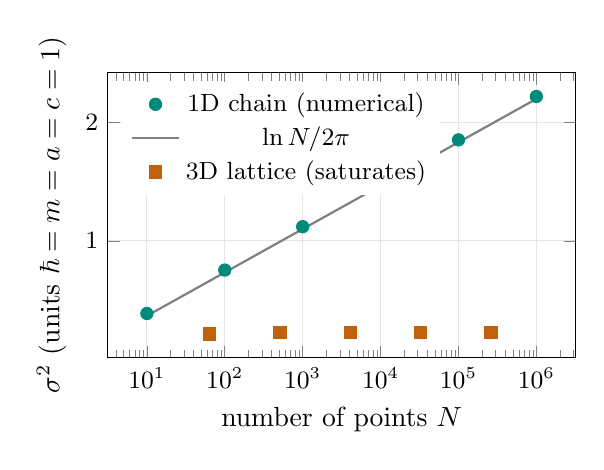
\begin{tikzpicture}
\begin{axis}[width=0.62\textwidth,height=5.2cm,xmode=log,xlabel={number of points $N$},ylabel={$\sigma^2$ (units $\hbar=m=a=c=1$)},
  legend pos=north west,legend style={font=\small,draw=none},grid=major,grid style={gray!20},tick label style={font=\small}]
\addplot[only marks,mark=*,mark size=2.2pt,bandA] coordinates {(10,0.3862)(100,0.7529)(1000,1.1194)(10000,1.4859)(100000,1.8523)(1000000,2.2188)};
\addlegendentry{1D chain (numerical)}
\addplot[domain=10:1000000,samples=40,thick,gray] {ln(x)/(2*pi)};
\addlegendentry{$\ln N/2\pi$}
\addplot[only marks,mark=square*,mark size=2.2pt,bandB] coordinates {(64,0.2140)(512,0.2242)(4096,0.2268)(32768,0.2275)(262144,0.2276)};
\addlegendentry{3D lattice (saturates)}
\end{axis}
\end{tikzpicture}
\caption{Zero-point positional blur of a point in a quantum lattice. In one dimension it grows logarithmically with system size; in three dimensions it saturates.}
\label{fig:blur}
\end{figure}

\paragraph{What it shows, and what it does not.} The blur of a point is a \emph{collective} property, fixed by the spectrum of modes the point is coupled to (system size, dimension). The linewidth of an atom is likewise fixed by the field modes it couples to. That is the extent of the analogy. It is \emph{not} true here that ``isolated means sharp'': an isolated, unpinned point is a free particle and is infinitely blurry, and with an on-site pin coupling \emph{reduces} the blur. The Lorentzian line shape is not reproduced. The model is a crystal with a rest frame and does nothing for Lorentz invariance. With $\hbar/mc=a=\lP$ the blur across the observable universe is only $\sigma\approx4.7\,\lP$. \ours{} Curiously, $\ln N\simeq\ln(L/\lP)$ is the same logarithm as the rapidity cutoff of Sec.~6. Both come from the scale-free $1/k$ behaviour of massless $1+1$ fields, and we attach no significance to it yet.

\section{A finite universe as a rapidity cutoff}
\ours{} A neighbour at proper time $\tau$ and rapidity $\eta$ lies at spatial distance $r=\tau\sinh\eta\approx(\tau/2)e^\eta$. In a universe of size $L$, $\eta\le\eta_{\max}\approx\ln(2L/\tau)$. With $L\approx4.4\times10^{26}$\,m and $\tau\sim\lP$, $L/\lP\approx2.7\times10^{61}$ and $\eta_{\max}\approx142$.
\begin{itemize}[leftmargin=*]
\item $1+1$: one link per unit rapidity gives $\approx2\eta_{\max}\approx280$ future links per point.
\item $3+1$: $d^4x=\tau^3\sinh^2\!\eta\,d\tau\,d\eta\,d\Omega$, the causal interval has volume $\pi\tau^4/24$, and $\int\sinh^2\eta\,d\eta\,d\Omega\approx\frac\pi2e^{2\eta_{\max}}$. Therefore
\begin{equation}
N_{\rm links}\approx2\pi\rho L^2\int_0^\infty\tau\,e^{-\rho\pi\tau^4/24}d\tau=\frac{\pi\sqrt{24}}{2}\Big(\frac{L}{\lP}\Big)^2\approx7.7\,(L/\lP)^2\sim10^{124}.
\end{equation}
\end{itemize}
The price is a preferred frame. A compact universe has a global rest frame~\cite{BarrowLevin01}, and we already observe a cosmological one, that of the CMB. The proposal is that Lorentz symmetry is exact for rapidities $\eta\ll\eta_{\max}\approx142$. The largest rapidity ever observed, a $\sim3\times10^{20}$\,eV cosmic-ray proton, is $\eta\approx27$. A literature search did not find this framing stated explicitly. It may well exist under other names.

\paragraph{Finite does not mean local.} Links lie near the light cone, out to cosmological distances. The emission of a photon in a distant galaxy and its absorption in an eye are nearly null-separated, so in this picture they are almost neighbours. The non-locality is light-cone-shaped. All links are timelike, so causality (no superluminal signalling) is preserved by construction.

\section{A point budget: expansion creates, gravity destroys}
\ours{} If point density $\rho$ is fixed (``Number $=$ Volume''~\cite{Surya19}), then point conservation $\partial_t\rho+\nabla\!\cdot(\rho\mathbf v)=s$ implies a creation rate $s=\rho\,\nabla\!\cdot\mathbf v$.
\begin{itemize}[leftmargin=*]
\item Hubble flow $\mathbf v=H\mathbf r$: $\nabla\!\cdot\mathbf v=3H$. Each point spawns new points at rate $3H$, or $3Ht_{\rm P}\approx3.6\times10^{-61}$ per Planck time today.
\item River model of a black hole~\cite{HamiltonLisle08}, $\mathbf v=-\sqrt{2GM/r}\,\hat{\mathbf r}$: $\nabla\!\cdot\mathbf v=-\tfrac32\sqrt{2GM/r^3}$, so points are destroyed. At the Earth's surface the rate is $\approx2.6\times10^{-3}\,\mathrm{s}^{-1}$. The sink is distributed through space rather than located in the matter, unlike Riemann's 19th-century aether-sink picture.
\end{itemize}
This connects to the sequential growth dynamics of causal sets~\cite{RideoutSorkin00}, in which time passing is the birth of new elements, to steady-state cosmology (creation of matter rather than of points), and to Sorkin's $\Lambda\sim1/\sqrt N$, which decreases as $N$ grows~\cite{ADGS04}. \emph{Main objection:} $\nabla\!\cdot\mathbf v$ is the expansion of a chosen family of observers, so a fixed-density picture needs a preferred congruence, which is an aether again~\cite{JacobsonMattingly01}.

\section{Discussion}
\subsection{Is this causal set theory?}
Partly. Several of our steps independently reached causal-set results: links, infinite valency, the dilemma, Number $=$ Volume, growth. The starting points and commitments differ, however.

\begin{center}
\small
\begin{tabular}{@{}>{\raggedright\arraybackslash}p{3.0cm}>{\raggedright\arraybackslash}p{5.3cm}>{\raggedright\arraybackslash}p{5.7cm}@{}}
\toprule
 & Causal sets & This notebook \\
\midrule
Starting picture & random sprinkling + causal order & regular crystal + quantum blur \\
Points & fundamental, no position & have a (blurred) position \\
Neighbours & links (empty interval) & ``one tick''; ends up equal to links \\
Lorentz invariance & exact, statistical & exact up to $\eta_{\max}$; cosmological frame accepted \\
Non-locality & accepted, infinite valency & accepted, finite but huge valency \\
Growth & sequential growth dynamics & point budget tied to flows \\
Background & none & implicitly present (blur, flow, density) \\
\bottomrule
\end{tabular}
\end{center}

\noindent The last row is the most important difference and our biggest weakness. A blur is a blur \emph{in} some space, and a flow is a flow \emph{relative to} something. Our picture leans on a background that GR teaches us to avoid. It is closer to a hybrid of causal sets with Einstein-aether or analog gravity~\cite{Unruh81} than to causal sets proper.

\subsection{Bell non-locality}
\est{} Bell correlations involve \emph{spacelike}-separated measurements $A,B$, which links never join. In the link graph $A$ and $B$ are two hops apart, through the common past (source) or the common future (comparison). Bell's theorem excludes classical common-cause stories through the past. The future route corresponds to retrocausal models. \lit{} The mainstream ``entanglement $\leftrightarrow$ connectivity'' programme is~\cite{VanRaamsdonk10,MaldacenaSusskind13}. We have no result here, only a question.

\subsection{The cosmological constant}
\lit{} Measured $\rho_\Lambda\approx6\times10^{-27}$\,kg\,m$^{-3}$ is $\sim10^{-123}$ of the Planck density, while summing zero-point energies $\tfrac12\hbar\omega$ (as in Sec.~5) to the Planck scale predicts roughly the Planck density. Sorkin's heuristic $\Lambda\sim1/\sqrt V$ from Poisson fluctuations in the number of points predicted the right order of magnitude before 1998~\cite{Surya19,ADGS04}, though it has been strongly constrained since~\cite{Barrow06,DNY23}. \emph{We offer no new hint.} The coincidence $(L/\lP)^2\sim10^{122}$ in Sec.~6 is numerology, since every dimensionless combination of $L$ and $\lP$ is a power of $10^{61}$. The point budget gives a narrative for why $N$ grows, but no number.

\section{Limitations}
\begin{enumerate}[leftmargin=*,itemsep=1pt]
\item No dynamics: nothing here produces Einstein's equations, or even Newtonian gravity.
\item Background dependence (Sec.~8.1).
\item The finite-universe cutoff is unobservable by construction ($\eta_{\max}\gg27$) and so, as stated, makes no prediction.
\item The point budget is slicing-dependent until it is formulated covariantly.
\item Most calculations are in $1+1$ dimensions; $3+1$ changes counts qualitatively (exponential vs.\ linear growth in rapidity).
\item Literature searches were brief; \ours{} items may be known.
\end{enumerate}

\section{Open questions for the next session}
\begin{enumerate}[leftmargin=*,itemsep=1pt]
\item Does Poisson-random point \emph{creation} reproduce Sorkin's $\sqrt N$ fluctuations naturally?
\item Is $\eta_{\max}$ set by the Hubble radius or by the event horizon, and does it evolve observably?
\item Can the point budget be made covariant, perhaps using the causal-set count of elements in causal intervals instead of a velocity field?
\item Can link-graph distance carry anything Bell-relevant beyond ordinary QM?
\item A faithful linewidth analogue: a probe point coupled to the chain as a bath.
\end{enumerate}

\begin{thebibliography}{99}\small
\bibitem{BLMS87} L.~Bombelli, J.~Lee, D.~Meyer, R.~D.~Sorkin, ``Space-time as a causal set'', Phys.\ Rev.\ Lett.\ 59, 521 (1987).
\bibitem{AJL05} J.~Ambj{\o}rn, J.~Jurkiewicz, R.~Loll, ``Spectral dimension of the universe is scale dependent'', Phys.\ Rev.\ Lett.\ 95, 171301 (2005), hep-th/0505113.
\bibitem{Burago} D.~Burago, ``Periodic metrics'' (1990s); see the statement in arXiv:1104.4460.
\bibitem{Weyl} H.~Weyl, \emph{Philosophy of Mathematics and Natural Science} (1949), the tile argument.
\bibitem{VahidiAslWierman} M.~Q.~Vahidi-Asl, J.~C.~Wierman, first-passage percolation on the Voronoi tessellation and Delaunay triangulation, in \emph{Random Graphs 87} (1990); shape result in \emph{Random Graphs 89} (1992).
\bibitem{Surya19} S.~Surya, ``The causal set approach to quantum gravity'', Living Rev.\ Rel.\ (2019), arXiv:1903.11544.
\bibitem{Sorkin11} R.~D.~Sorkin et al., ``Directions in causal set quantum gravity'', arXiv:1103.6272.
\bibitem{Schild48} A.~Schild, ``Discrete space-time and integral Lorentz transformations'', Phys.\ Rev.\ 73, 414 (1948); Canad.\ J.\ Math.\ 1, 29 (1949).
\bibitem{BHS06} L.~Bombelli, J.~Henson, R.~D.~Sorkin, ``Discreteness without symmetry breaking: a theorem'', gr-qc/0605006.
\bibitem{Sorkin07} R.~D.~Sorkin, ``Does locality fail at intermediate length-scales?'', gr-qc/0703099.
\bibitem{KosteleckySamuel89} V.~A.~Kosteleck\'y, S.~Samuel, ``Spontaneous breaking of Lorentz symmetry in string theory'', Phys.\ Rev.\ D 39, 683 (1989).
\bibitem{JacobsonMattingly01} T.~Jacobson, D.~Mattingly, ``Gravity with a dynamical preferred frame'', gr-qc/0007031.
\bibitem{BarrowLevin01} J.~D.~Barrow, J.~Levin, ``The twin paradox in compact spaces'', Phys.\ Rev.\ A 63, 044104 (2001).
\bibitem{HamiltonLisle08} A.~J.~S.~Hamilton, J.~P.~Lisle, ``The river model of black holes'', Am.\ J.\ Phys.\ 76, 519 (2008).
\bibitem{RideoutSorkin00} D.~P.~Rideout, R.~D.~Sorkin, ``A classical sequential growth dynamics for causal sets'', Phys.\ Rev.\ D 61, 024002 (2000).
\bibitem{ADGS04} M.~Ahmed, S.~Dodelson, P.~Greene, R.~D.~Sorkin, ``Everpresent $\Lambda$'', Phys.\ Rev.\ D 69, 103523 (2004).
\bibitem{Barrow06} J.~D.~Barrow, ``A strong constraint on ever-present Lambda'', gr-qc/0612128.
\bibitem{DNY23} A.~Das, A.~Nasiri, Y.~K.~Yazdi, ``Aspects of Everpresent $\Lambda$'' I \& II, arXiv:2304.03819, 2307.13743.
\bibitem{Unruh81} W.~G.~Unruh, ``Experimental black-hole evaporation?'', Phys.\ Rev.\ Lett.\ 46, 1351 (1981).
\bibitem{VanRaamsdonk10} M.~Van Raamsdonk, ``Building up spacetime with quantum entanglement'' (2010), arXiv:1005.3035.
\bibitem{MaldacenaSusskind13} J.~Maldacena, L.~Susskind, ``Cool horizons for entangled black holes'', arXiv:1306.0533.
\end{thebibliography}
\end{document}
